\documentclass[18pt, a3paper, portrait]{tikzposter}
\usepackage[utf8]{inputenc}

\makeatletter
\def\title#1{\gdef\@title{\scalebox{\TP@titletextscale}{%
\begin{minipage}[t]{\linewidth}
\centering
#1
\par
\vspace{0.5em}
\end{minipage}%
}}}
\makeatother

\title{Data Exploration and Conclusion}
\author{Yohann Jacob Sandvik}
\date{\today}
\institute{Institute of Electronic Systems - NTNU}
 
\usepackage{blindtext}
\usepackage{comment}
\usepackage{tikz} % To make cool diagrams
\usepackage{booktabs} % For fancy tables

\newcommand{\ra}[1]{\renewcommand{\arraystretch}{#1}} % Something about allowing more space between rows in fancy tables.
 
\usetheme{Envelope}
 
\begin{document}
 
\maketitle 

%% Dataset description
\begin{columns}
    \column{0.5}
    \block{All Values Associated with A Turbine}
    {
        \begin{tikzfigure}
            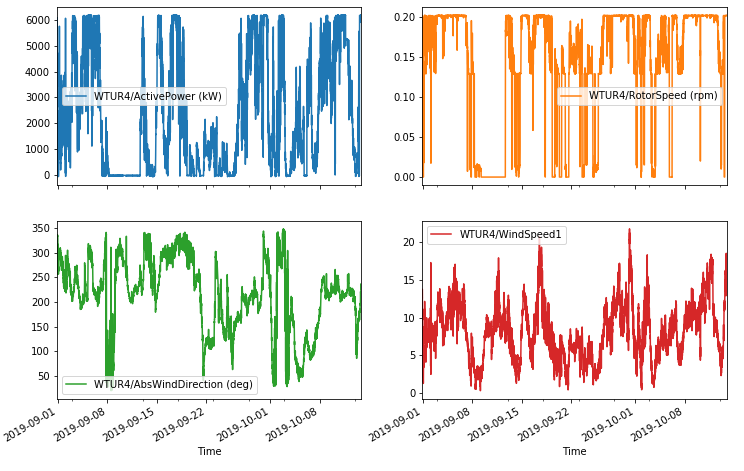
\includegraphics[width=0.45\textwidth]{images/one_turbine_all_vals.png}
        \end{tikzfigure}
    }
 
    \column{0.5}
    \block{Dataset Description}
    {
        \begin{itemize}
            \item This dataset is taken from a wind farm in Norway with 13 wind turbines.
            \item Each turbine can be viewed as a multivariate time series, with four dimensions: active power produced by a turbine in kilowatts, wind speed measured in front of the blades in meters per second, the rotational speed of the rotor in rpm and the absolute direction of the wind speed in degrees.
            \item The values are sampled every five minutes from the 31. of August 2019 00:00 until the 13. of September 2019 21:55, which totals 12239 samples per univariate time series and 48956 samples per wind turbine.
            \item The dataset chosen does not have any missing values, so there was no requirement for estimating missing values.
        \end{itemize}
        \vspace{9.5cm}
    }
\end{columns}

%% Describe tool and show figures of explained variance, and reconstruction error
\begin{columns}
    \column{0.5}
    \block{Cumulative Explained Variance and Reconstruction Error}
    {
        \begin{tikzfigure}
            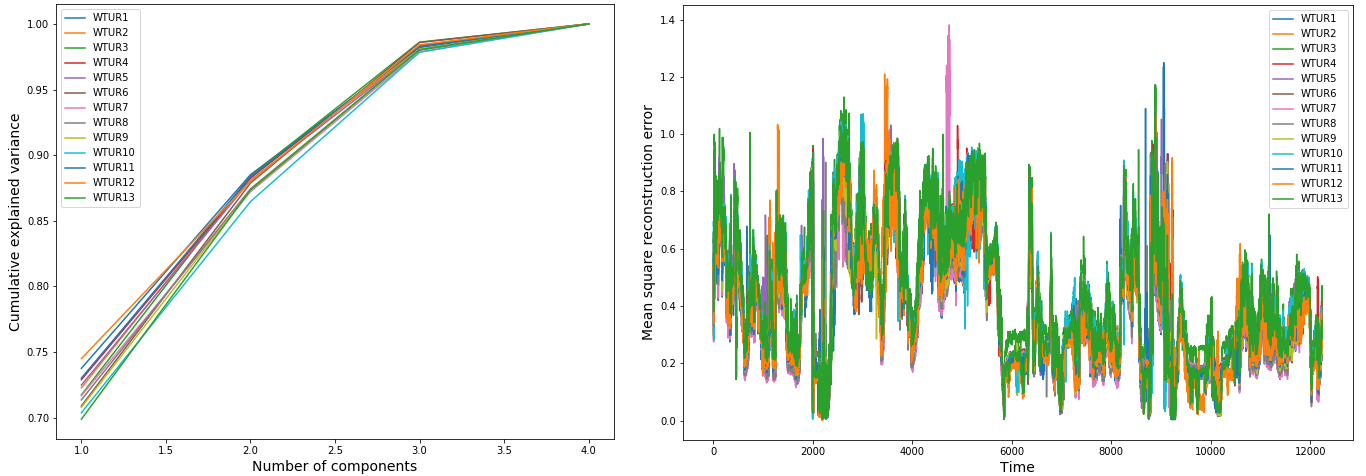
\includegraphics[width=0.45\textwidth]{images/two_besides.png}
        \end{tikzfigure}
    }
 
    \column{0.5}
    \block{What Can PCA Do?}
    {
        \begin{itemize}
            \item The total variance is the sum of the variences of the individual principal components.
            \item The explained variance of a principal component is the ratio of the variance of said component to the total variance of all the principal components, and the cumulative explained variance of $n$ principal components is the sum of the explained variance of the $n$ first principal components.
            \item The rightmost plot shows the cumulative explained variance of each turbine for a given number of principle components.
            \item The leftmost plot shows the total MSE of the reconstructed time series associated with the different wind turbines.
            \item From the figure one can see that all the cumulative explained variance curves, and reconstruction error curves follow more or less the same shape, with the exception of turbine seven that has a slight spike at round about 5000 samples. 
        \end{itemize}
    }
\end{columns}

%% Artificial perturbation pics
\begin{columns}
    \column{0.25}
    \block{Perturbation}
    {
        \begin{tikzfigure}
            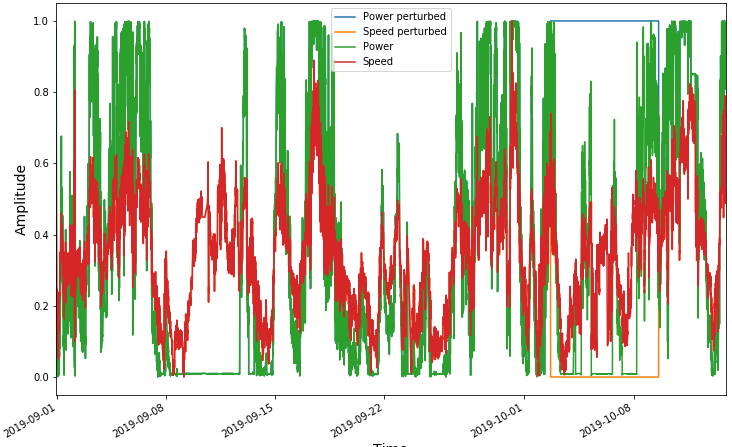
\includegraphics[width=0.21\textwidth]{images/perturbed_vs_unperturbed.png}
        \end{tikzfigure}
    }

    \column{0.25}
    \block{CEV}
    {
        \begin{tikzfigure}
            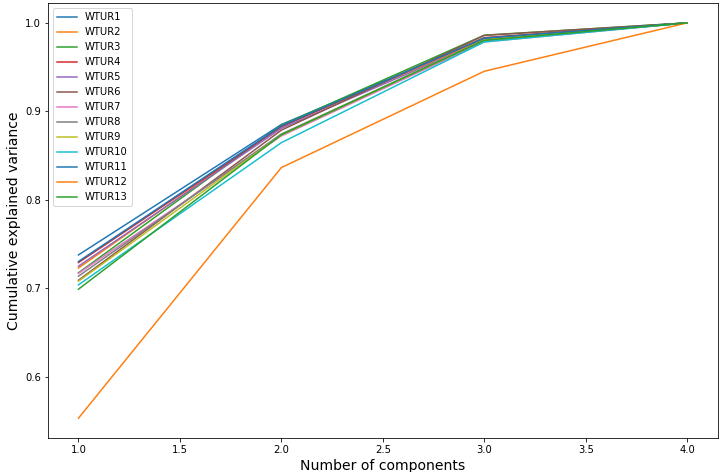
\includegraphics[width=0.21\textwidth]{images/explained_variance_perturbed.png}
        \end{tikzfigure}
    }

    \column{0.25}
    \block{Pert vs. Unpert}
    {
        \begin{tikzfigure}
            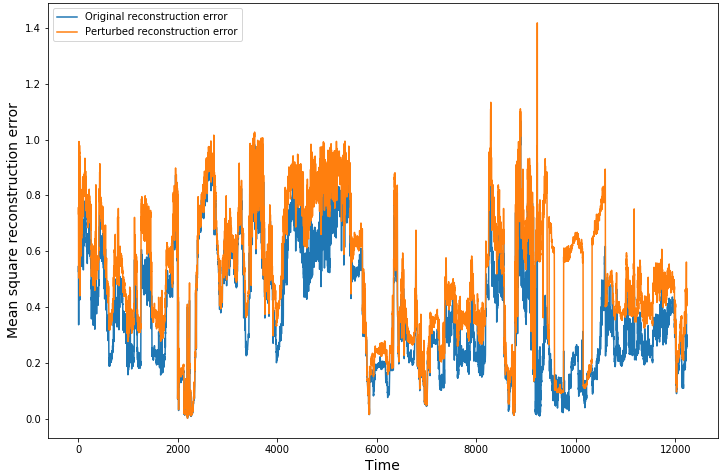
\includegraphics[width=0.21\textwidth]{images/pert_vs_unpert_reconstruction_error.png}
        \end{tikzfigure}
    }

    \column{0.25}
    \block{Reconstruction Error}
    {
        \begin{tikzfigure}
            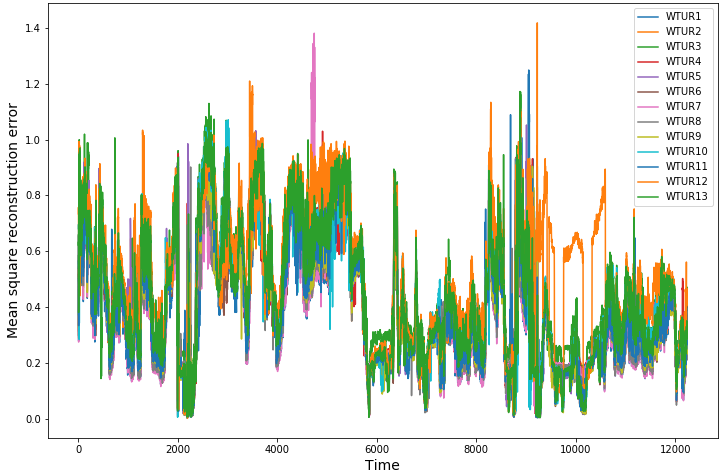
\includegraphics[width=0.21\textwidth]{images/reconstruction_error_perturbed.png}
        \end{tikzfigure}
    }
\end{columns}

%% Discussion 
\block{Discussion}
{
    \begin{itemize}
        \item From the cumulative explained variance plot, it is possible to see that artifical perturbation is quite evident.
        \item The reconstruction error also shows the artificial perturbation.
        \item The most interesting observation might be that the reconstruction error caused by artificial perturbation could yield a ''threshold'' as to what can be considered anomalous behaviour.
        \item As for example the peak in reconstruction error of turbine seven at around 5000 samples.
    \end{itemize}
}

%% Conclusion and future work
\block{Conclusion}
{
    The methods chosen to be most relevant to be explored in a master thesis are:
    \begin{itemize}
        \item Feature extraction using PCA, and clustering in reduced feature space.
        \item Model-based time series representation using a univariate ARMA model, and possibly a multivariate vector AR model.
        \item Since there are many open-source python implementations of different clustering algorithms, the only restriction set on which clustering algorithms to test is ease of implementation. So algorithms such as Self-organizing maps are excluded.
    \end{itemize}
}
\end{document}


